\hypertarget{Classes_8h}{
\section{Classes.h File Reference}
\label{Classes_8h}\index{Classes.h@{Classes.h}}
}


This graph shows which files directly or indirectly include this file:\begin{figure}[H]
\begin{center}
\leavevmode
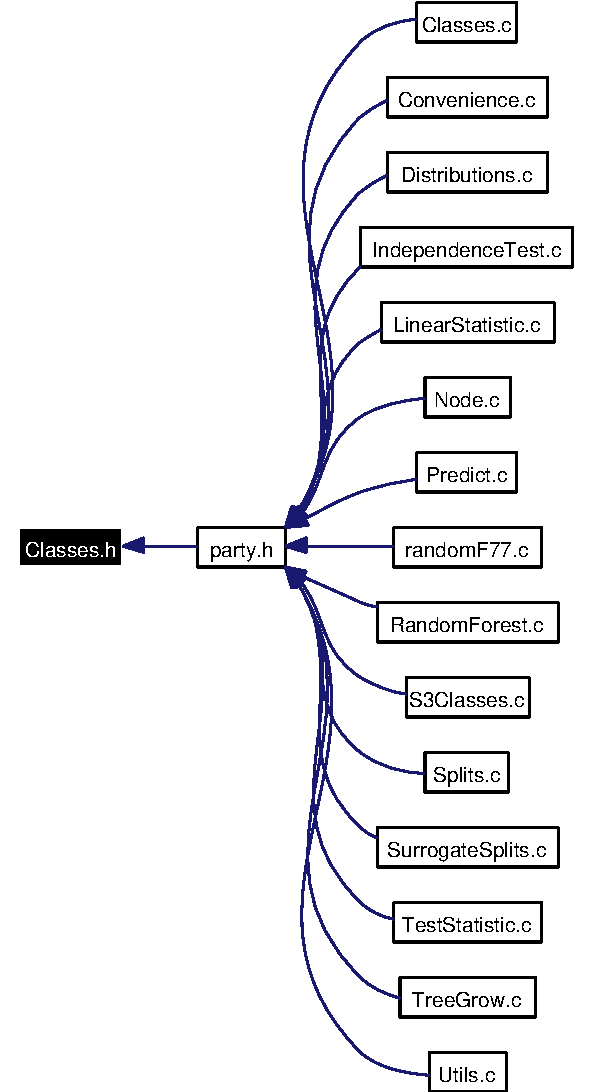
\includegraphics[width=159pt]{Classes_8h__dep__incl}
\end{center}
\end{figure}
\subsection*{Functions}
\begin{CompactItemize}
\item 
int \hyperlink{Classes_8h_a59}{get\_\-dimension} (SEXP object)
\item 
int \hyperlink{Classes_8h_a60}{get\_\-teststattype} (SEXP object)
\item 
double \hyperlink{Classes_8h_a61}{get\_\-tol} (SEXP object)
\item 
int \hyperlink{Classes_8h_a62}{get\_\-pvalue} (SEXP object)
\item 
int \hyperlink{Classes_8h_a63}{get\_\-maxpts} (SEXP object)
\item 
double \hyperlink{Classes_8h_a64}{get\_\-abseps} (SEXP object)
\item 
double \hyperlink{Classes_8h_a65}{get\_\-releps} (SEXP object)
\item 
double \hyperlink{Classes_8h_a66}{get\_\-minsplit} (SEXP object)
\item 
double \hyperlink{Classes_8h_a67}{get\_\-minprob} (SEXP object)
\item 
double \hyperlink{Classes_8h_a68}{get\_\-minbucket} (SEXP object)
\item 
SEXP \hyperlink{Classes_8h_a69}{get\_\-transformation} (SEXP object, int variable)
\item 
SEXP \hyperlink{Classes_8h_a70}{get\_\-jointtransf} (SEXP object)
\item 
SEXP \hyperlink{Classes_8h_a71}{get\_\-variable} (SEXP object, int variable)
\item 
int \hyperlink{Classes_8h_a72}{is\_\-nominal} (SEXP object, int variable)
\item 
int \hyperlink{Classes_8h_a73}{is\_\-ordinal} (SEXP object, int variable)
\item 
int \hyperlink{Classes_8h_a74}{is\_\-censored} (SEXP object, int variable)
\item 
int \hyperlink{Classes_8h_a75}{has\_\-missings} (SEXP object, int variable)
\item 
SEXP \hyperlink{Classes_8h_a76}{get\_\-missings} (SEXP object, int variable)
\item 
SEXP \hyperlink{Classes_8h_a77}{get\_\-ordering} (SEXP object, int variable)
\item 
SEXP \hyperlink{Classes_8h_a78}{get\_\-levels} (SEXP object, int variable)
\item 
SEXP \hyperlink{Classes_8h_a79}{get\_\-scores} (SEXP object, int variable)
\item 
SEXP \hyperlink{Classes_8h_a80}{get\_\-which\-NA} (SEXP object, int variable)
\item 
SEXP \hyperlink{Classes_8h_a81}{get\_\-varmemory} (SEXP object, int variable)
\item 
SEXP \hyperlink{Classes_8h_a82}{get\_\-var\-Mmemory} (SEXP object, int variable)
\item 
SEXP \hyperlink{Classes_8h_a83}{get\_\-Mscorematrix} (SEXP object, int variable)
\item 
int \hyperlink{Classes_8h_a84}{get\_\-nobs} (SEXP object)
\item 
int \hyperlink{Classes_8h_a85}{get\_\-ninputs} (SEXP object)
\item 
SEXP \hyperlink{Classes_8h_a86}{get\_\-weights} (SEXP object, int variable)
\item 
int \hyperlink{Classes_8h_a87}{get\_\-testtype} (SEXP object)
\item 
int \hyperlink{Classes_8h_a88}{get\_\-nresample} (SEXP object)
\item 
SEXP \hyperlink{Classes_8h_a89}{get\_\-varctrl} (SEXP object)
\item 
SEXP \hyperlink{Classes_8h_a90}{get\_\-splitctrl} (SEXP object)
\item 
SEXP \hyperlink{Classes_8h_a91}{get\_\-gtctrl} (SEXP object)
\item 
double \hyperlink{Classes_8h_a92}{get\_\-mincriterion} (SEXP object)
\item 
int \hyperlink{Classes_8h_a93}{get\_\-randomsplits} (SEXP object)
\item 
int \hyperlink{Classes_8h_a94}{get\_\-mtry} (SEXP object)
\item 
SEXP \hyperlink{Classes_8h_a95}{get\_\-dontuse} (SEXP object)
\item 
SEXP \hyperlink{Classes_8h_a96}{get\_\-dontusetmp} (SEXP object)
\item 
int \hyperlink{Classes_8h_a97}{get\_\-stump} (SEXP object)
\item 
int \hyperlink{Classes_8h_a98}{get\_\-maxsurrogate} (SEXP object)
\item 
SEXP \hyperlink{Classes_8h_a99}{get\_\-tgctrl} (SEXP object)
\item 
SEXP \hyperlink{Classes_8h_a100}{get\_\-splitstatistics} (SEXP object)
\item 
int \hyperlink{Classes_8h_a101}{get\_\-savesplitstats} (SEXP object)
\end{CompactItemize}
\subsection*{Variables}
\begin{CompactItemize}
\item 
SEXP \hyperlink{Classes_8h_a0}{PL2\_\-expectation\-Sym}
\item 
SEXP \hyperlink{Classes_8h_a1}{PL2\_\-covariance\-Sym}
\item 
SEXP \hyperlink{Classes_8h_a2}{PL2\_\-linearstatistic\-Sym}
\item 
SEXP \hyperlink{Classes_8h_a3}{PL2\_\-expcovinf\-Sym}
\item 
SEXP \hyperlink{Classes_8h_a4}{PL2\_\-expcovinfss\-Sym}
\item 
SEXP \hyperlink{Classes_8h_a5}{PL2\_\-sumweights\-Sym}
\item 
SEXP \hyperlink{Classes_8h_a6}{PL2\_\-dimension\-Sym}
\item 
SEXP \hyperlink{Classes_8h_a7}{PL2\_\-MPinv\-Sym}
\item 
SEXP \hyperlink{Classes_8h_a8}{PL2\_\-rank\-Sym}
\item 
SEXP \hyperlink{Classes_8h_a9}{PL2\_\-svd\-Sym}
\item 
SEXP \hyperlink{Classes_8h_a10}{PL2\_\-svdmem\-Sym}
\item 
SEXP \hyperlink{Classes_8h_a11}{PL2\_\-method\-Sym}
\item 
SEXP \hyperlink{Classes_8h_a12}{PL2\_\-jobu\-Sym}
\item 
SEXP \hyperlink{Classes_8h_a13}{PL2\_\-jobv\-Sym}
\item 
SEXP \hyperlink{Classes_8h_a14}{PL2\_\-u\-Sym}
\item 
SEXP \hyperlink{Classes_8h_a15}{PL2\_\-v\-Sym}
\item 
SEXP \hyperlink{Classes_8h_a16}{PL2\_\-s\-Sym}
\item 
SEXP \hyperlink{Classes_8h_a17}{PL2\_\-p\-Sym}
\item 
SEXP \hyperlink{Classes_8h_a18}{PL2\_\-teststattype\-Sym}
\item 
SEXP \hyperlink{Classes_8h_a19}{PL2\_\-pvalue\-Sym}
\item 
SEXP \hyperlink{Classes_8h_a20}{PL2\_\-tol\-Sym}
\item 
SEXP \hyperlink{Classes_8h_a21}{PL2\_\-maxpts\-Sym}
\item 
SEXP \hyperlink{Classes_8h_a22}{PL2\_\-abseps\-Sym}
\item 
SEXP \hyperlink{Classes_8h_a23}{PL2\_\-releps\-Sym}
\item 
SEXP \hyperlink{Classes_8h_a24}{PL2\_\-minsplit\-Sym}
\item 
SEXP \hyperlink{Classes_8h_a25}{PL2\_\-minbucket\-Sym}
\item 
SEXP \hyperlink{Classes_8h_a26}{PL2\_\-minprob\-Sym}
\item 
SEXP \hyperlink{Classes_8h_a27}{PL2\_\-variables\-Sym}
\item 
SEXP \hyperlink{Classes_8h_a28}{PL2\_\-transformations\-Sym}
\item 
SEXP \hyperlink{Classes_8h_a29}{PL2\_\-is\_\-nominal\-Sym}
\item 
SEXP \hyperlink{Classes_8h_a30}{PL2\_\-is\_\-ordinal\-Sym}
\item 
SEXP \hyperlink{Classes_8h_a31}{PL2\_\-is\_\-censored\-Sym}
\item 
SEXP \hyperlink{Classes_8h_a32}{PL2\_\-ordering\-Sym}
\item 
SEXP \hyperlink{Classes_8h_a33}{PL2\_\-levels\-Sym}
\item 
SEXP \hyperlink{Classes_8h_a34}{PL2\_\-scores\-Sym}
\item 
SEXP \hyperlink{Classes_8h_a35}{PL2\_\-has\_\-missings\-Sym}
\item 
SEXP \hyperlink{Classes_8h_a36}{PL2\_\-which\-NASym}
\item 
SEXP \hyperlink{Classes_8h_a37}{PL2\_\-jointtransf\-Sym}
\item 
SEXP \hyperlink{Classes_8h_a38}{PL2\_\-nobs\-Sym}
\item 
SEXP \hyperlink{Classes_8h_a39}{PL2\_\-ninputs\-Sym}
\item 
SEXP \hyperlink{Classes_8h_a40}{PL2\_\-linexpcov2sample\-Sym}
\item 
SEXP \hyperlink{Classes_8h_a41}{PL2\_\-weights\-Sym}
\item 
SEXP \hyperlink{Classes_8h_a42}{PL2\_\-varmemory\-Sym}
\item 
SEXP \hyperlink{Classes_8h_a43}{PL2\_\-var\-Mmemory\-Sym}
\item 
SEXP \hyperlink{Classes_8h_a44}{PL2\_\-Mscorematrices\-Sym}
\item 
SEXP \hyperlink{Classes_8h_a45}{PL2\_\-responses\-Sym}
\item 
SEXP \hyperlink{Classes_8h_a46}{PL2\_\-inputs\-Sym}
\item 
SEXP \hyperlink{Classes_8h_a47}{PL2\_\-testtype\-Sym}
\item 
SEXP \hyperlink{Classes_8h_a48}{PL2\_\-nresample\-Sym}
\item 
SEXP \hyperlink{Classes_8h_a49}{PL2\_\-varctrl\-Sym}
\item 
SEXP \hyperlink{Classes_8h_a50}{PL2\_\-splitctrl\-Sym}
\item 
SEXP \hyperlink{Classes_8h_a51}{PL2\_\-gtctrl\-Sym}
\item 
SEXP \hyperlink{Classes_8h_a52}{PL2\_\-mincriterion\-Sym}
\item 
SEXP \hyperlink{Classes_8h_a53}{PL2\_\-randomsplits\-Sym}
\item 
SEXP \hyperlink{Classes_8h_a54}{PL2\_\-mtry\-Sym}
\item 
SEXP \hyperlink{Classes_8h_a55}{PL2\_\-dontuse\-Sym}
\item 
SEXP \hyperlink{Classes_8h_a56}{PL2\_\-dontusetmp\-Sym}
\item 
SEXP \hyperlink{Classes_8h_a57}{PL2\_\-stump\-Sym}
\item 
SEXP \hyperlink{Classes_8h_a58}{PL2\_\-tgctrl\-Sym}
\end{CompactItemize}


\subsection{Function Documentation}
\hypertarget{Classes_8h_a64}{
\index{Classes.h@{Classes.h}!get_abseps@{get\_\-abseps}}
\index{get_abseps@{get\_\-abseps}!Classes.h@{Classes.h}}
\subsubsection[get\_\-abseps]{\setlength{\rightskip}{0pt plus 5cm}double get\_\-abseps (SEXP {\em object})}}
\label{Classes_8h_a64}




Definition at line 163 of file Classes.c.

References PL2\_\-abseps\-Sym.

Referenced by C\_\-Teststat\-Pvalue().\hypertarget{Classes_8h_a59}{
\index{Classes.h@{Classes.h}!get_dimension@{get\_\-dimension}}
\index{get_dimension@{get\_\-dimension}!Classes.h@{Classes.h}}
\subsubsection[get\_\-dimension]{\setlength{\rightskip}{0pt plus 5cm}int get\_\-dimension (SEXP {\em object})}}
\label{Classes_8h_a59}




Definition at line 143 of file Classes.c.

References PL2\_\-dimension\-Sym.

Referenced by C\_\-Conditional\-Pvalue(), C\_\-MLinear\-Statistic(), C\_\-Node(), C\_\-Test\-Statistic(), and R\_\-splitcategorical().\hypertarget{Classes_8h_a95}{
\index{Classes.h@{Classes.h}!get_dontuse@{get\_\-dontuse}}
\index{get_dontuse@{get\_\-dontuse}!Classes.h@{Classes.h}}
\subsubsection[get\_\-dontuse]{\setlength{\rightskip}{0pt plus 5cm}SEXP get\_\-dontuse (SEXP {\em object})}}
\label{Classes_8h_a95}




Definition at line 335 of file Classes.c.

References PL2\_\-dontuse\-Sym.

Referenced by C\_\-Global\-Test().\hypertarget{Classes_8h_a96}{
\index{Classes.h@{Classes.h}!get_dontusetmp@{get\_\-dontusetmp}}
\index{get_dontusetmp@{get\_\-dontusetmp}!Classes.h@{Classes.h}}
\subsubsection[get\_\-dontusetmp]{\setlength{\rightskip}{0pt plus 5cm}SEXP get\_\-dontusetmp (SEXP {\em object})}}
\label{Classes_8h_a96}




Definition at line 339 of file Classes.c.

References PL2\_\-dontusetmp\-Sym.

Referenced by C\_\-Global\-Test().\hypertarget{Classes_8h_a91}{
\index{Classes.h@{Classes.h}!get_gtctrl@{get\_\-gtctrl}}
\index{get_gtctrl@{get\_\-gtctrl}!Classes.h@{Classes.h}}
\subsubsection[get\_\-gtctrl]{\setlength{\rightskip}{0pt plus 5cm}SEXP get\_\-gtctrl (SEXP {\em object})}}
\label{Classes_8h_a91}




Definition at line 311 of file Classes.c.

References PL2\_\-gtctrl\-Sym.

Referenced by C\_\-Node().\hypertarget{Classes_8h_a70}{
\index{Classes.h@{Classes.h}!get_jointtransf@{get\_\-jointtransf}}
\index{get_jointtransf@{get\_\-jointtransf}!Classes.h@{Classes.h}}
\subsubsection[get\_\-jointtransf]{\setlength{\rightskip}{0pt plus 5cm}SEXP get\_\-jointtransf (SEXP {\em object})}}
\label{Classes_8h_a70}




Definition at line 189 of file Classes.c.

References PL2\_\-jointtransf\-Sym.\hypertarget{Classes_8h_a78}{
\index{Classes.h@{Classes.h}!get_levels@{get\_\-levels}}
\index{get_levels@{get\_\-levels}!Classes.h@{Classes.h}}
\subsubsection[get\_\-levels]{\setlength{\rightskip}{0pt plus 5cm}SEXP get\_\-levels (SEXP {\em object}, int {\em variable})}}
\label{Classes_8h_a78}




Definition at line 226 of file Classes.c.

References is\_\-nominal(), is\_\-ordinal(), and PL2\_\-levels\-Sym.

Referenced by C\_\-Node().

Here is the call graph for this function:\begin{figure}[H]
\begin{center}
\leavevmode
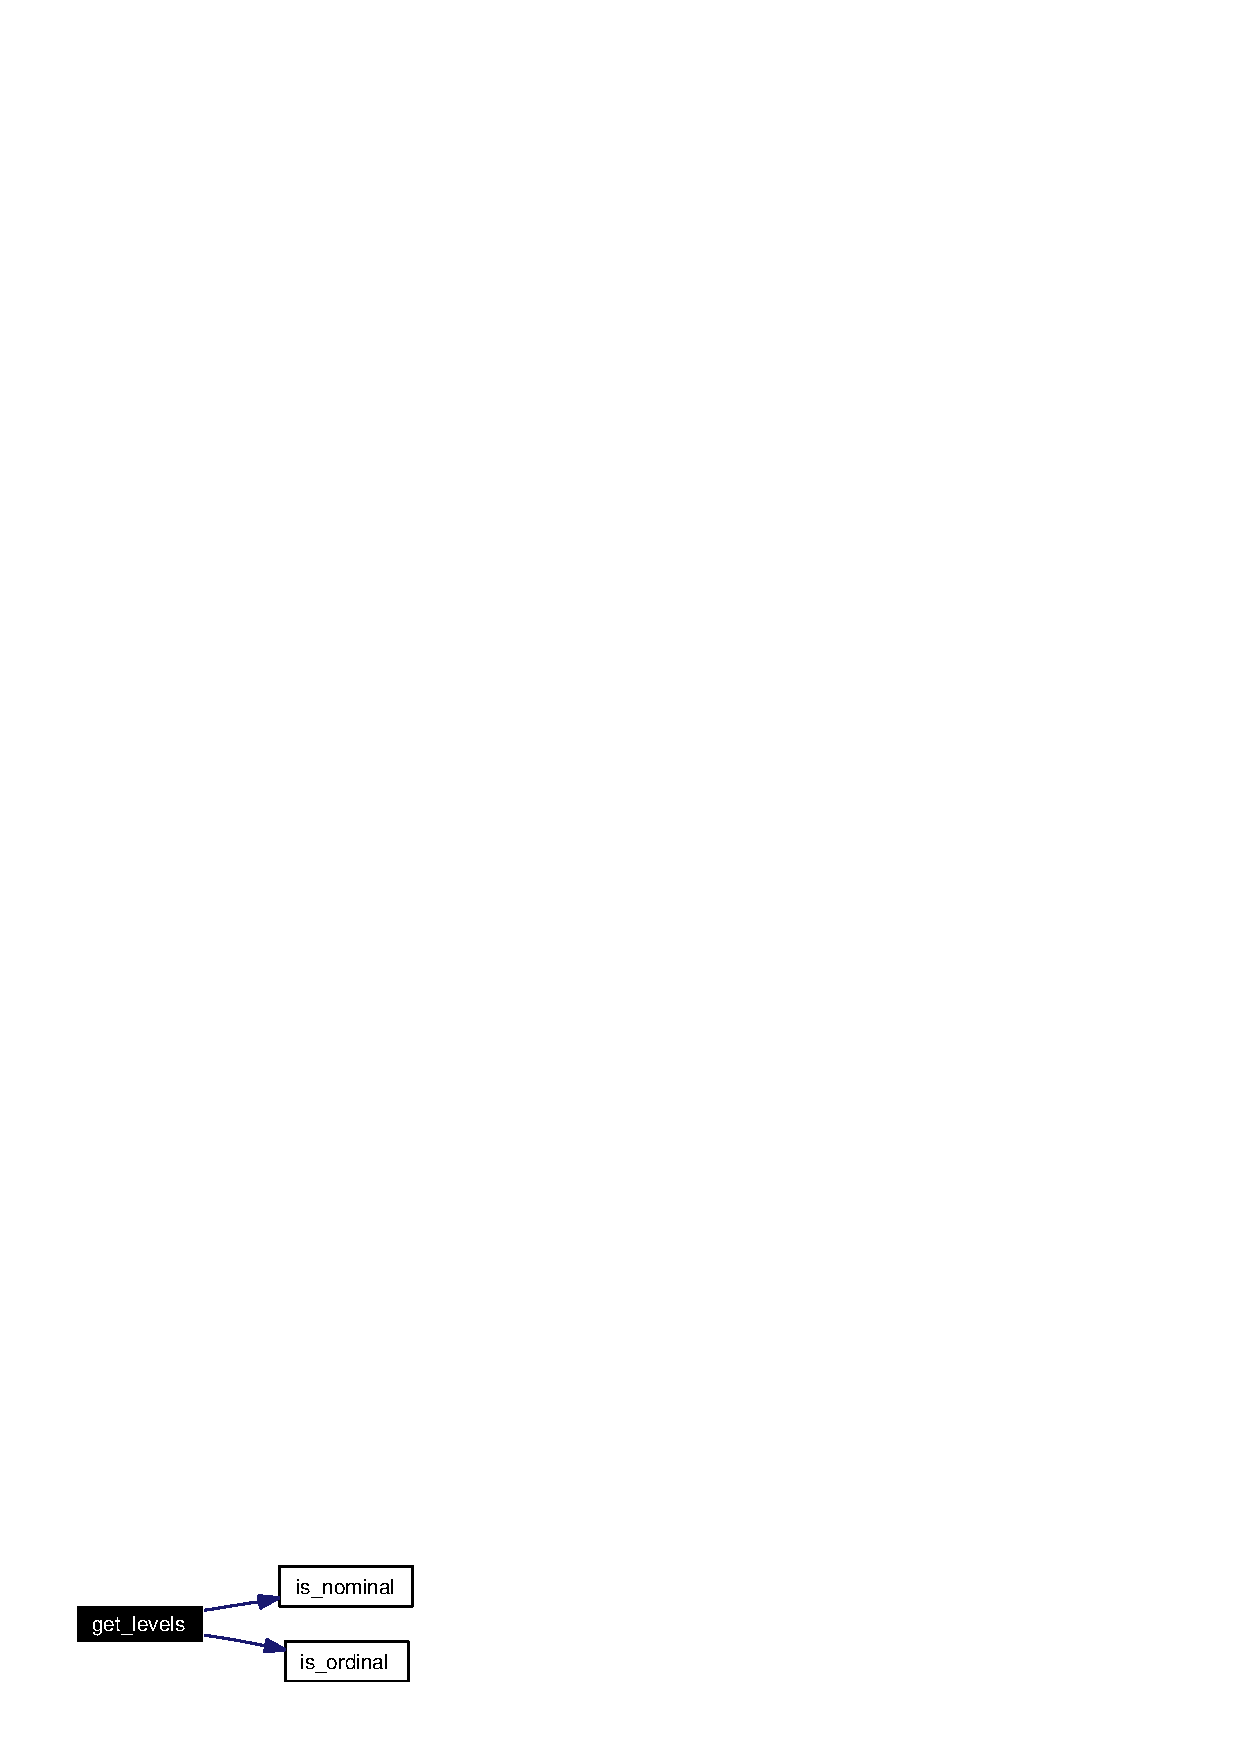
\includegraphics[width=104pt]{Classes_8h_a78_cgraph}
\end{center}
\end{figure}
\hypertarget{Classes_8h_a63}{
\index{Classes.h@{Classes.h}!get_maxpts@{get\_\-maxpts}}
\index{get_maxpts@{get\_\-maxpts}!Classes.h@{Classes.h}}
\subsubsection[get\_\-maxpts]{\setlength{\rightskip}{0pt plus 5cm}int get\_\-maxpts (SEXP {\em object})}}
\label{Classes_8h_a63}




Definition at line 159 of file Classes.c.

References PL2\_\-maxpts\-Sym.

Referenced by C\_\-Teststat\-Pvalue().\hypertarget{Classes_8h_a98}{
\index{Classes.h@{Classes.h}!get_maxsurrogate@{get\_\-maxsurrogate}}
\index{get_maxsurrogate@{get\_\-maxsurrogate}!Classes.h@{Classes.h}}
\subsubsection[get\_\-maxsurrogate]{\setlength{\rightskip}{0pt plus 5cm}int get\_\-maxsurrogate (SEXP {\em object})}}
\label{Classes_8h_a98}




Definition at line 323 of file Classes.c.

References PL2\_\-maxsurrogate\-Sym.

Referenced by C\_\-splitnode(), C\_\-surrogates(), C\_\-Tree\-Grow(), R\_\-Ensemble(), R\_\-Node(), and R\_\-Tree\-Grow().\hypertarget{Classes_8h_a68}{
\index{Classes.h@{Classes.h}!get_minbucket@{get\_\-minbucket}}
\index{get_minbucket@{get\_\-minbucket}!Classes.h@{Classes.h}}
\subsubsection[get\_\-minbucket]{\setlength{\rightskip}{0pt plus 5cm}double get\_\-minbucket (SEXP {\em object})}}
\label{Classes_8h_a68}




Definition at line 179 of file Classes.c.

References PL2\_\-minbucket\-Sym.

Referenced by C\_\-split().\hypertarget{Classes_8h_a92}{
\index{Classes.h@{Classes.h}!get_mincriterion@{get\_\-mincriterion}}
\index{get_mincriterion@{get\_\-mincriterion}!Classes.h@{Classes.h}}
\subsubsection[get\_\-mincriterion]{\setlength{\rightskip}{0pt plus 5cm}double get\_\-mincriterion (SEXP {\em object})}}
\label{Classes_8h_a92}




Definition at line 319 of file Classes.c.

References PL2\_\-mincriterion\-Sym.

Referenced by C\_\-Node().\hypertarget{Classes_8h_a67}{
\index{Classes.h@{Classes.h}!get_minprob@{get\_\-minprob}}
\index{get_minprob@{get\_\-minprob}!Classes.h@{Classes.h}}
\subsubsection[get\_\-minprob]{\setlength{\rightskip}{0pt plus 5cm}double get\_\-minprob (SEXP {\em object})}}
\label{Classes_8h_a67}




Definition at line 175 of file Classes.c.

References PL2\_\-minprob\-Sym.

Referenced by C\_\-split().\hypertarget{Classes_8h_a66}{
\index{Classes.h@{Classes.h}!get_minsplit@{get\_\-minsplit}}
\index{get_minsplit@{get\_\-minsplit}!Classes.h@{Classes.h}}
\subsubsection[get\_\-minsplit]{\setlength{\rightskip}{0pt plus 5cm}double get\_\-minsplit (SEXP {\em object})}}
\label{Classes_8h_a66}




Definition at line 171 of file Classes.c.

References PL2\_\-minsplit\-Sym.

Referenced by C\_\-Node().\hypertarget{Classes_8h_a76}{
\index{Classes.h@{Classes.h}!get_missings@{get\_\-missings}}
\index{get_missings@{get\_\-missings}!Classes.h@{Classes.h}}
\subsubsection[get\_\-missings]{\setlength{\rightskip}{0pt plus 5cm}SEXP get\_\-missings (SEXP {\em object}, int {\em variable})}}
\label{Classes_8h_a76}




Definition at line 249 of file Classes.c.

References has\_\-missings(), and PL2\_\-which\-NASym.

Referenced by C\_\-get\_\-node(), C\_\-Global\-Test(), C\_\-splitnode(), C\_\-splitsurrogate(), and C\_\-surrogates().

Here is the call graph for this function:\begin{figure}[H]
\begin{center}
\leavevmode
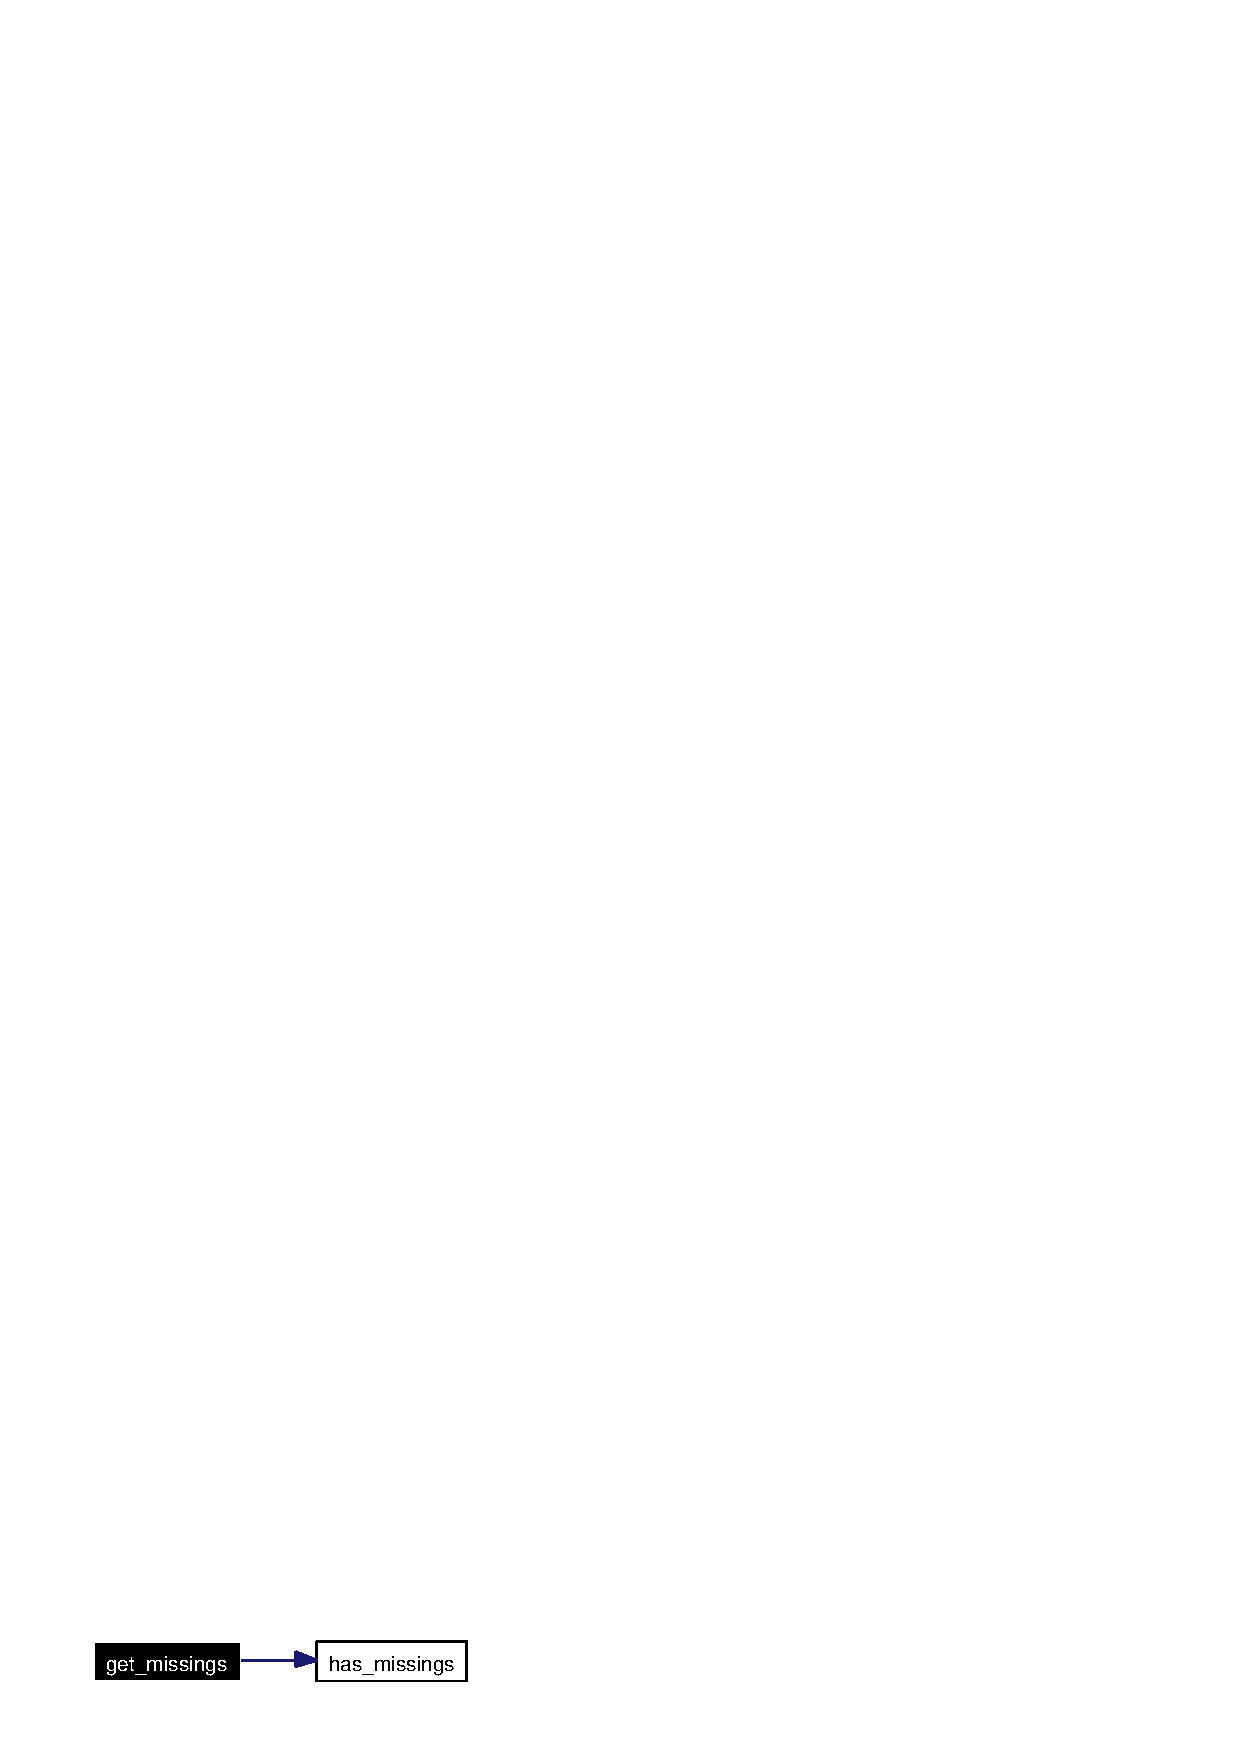
\includegraphics[width=116pt]{Classes_8h_a76_cgraph}
\end{center}
\end{figure}
\hypertarget{Classes_8h_a83}{
\index{Classes.h@{Classes.h}!get_Mscorematrix@{get\_\-Mscorematrix}}
\index{get_Mscorematrix@{get\_\-Mscorematrix}!Classes.h@{Classes.h}}
\subsubsection[get\_\-Mscorematrix]{\setlength{\rightskip}{0pt plus 5cm}SEXP get\_\-Mscorematrix (SEXP {\em object}, int {\em variable})}}
\label{Classes_8h_a83}




Definition at line 270 of file Classes.c.

References PL2\_\-Mscorematrices\-Sym.

Referenced by C\_\-Global\-Test(), and C\_\-Monte\-Carlo().\hypertarget{Classes_8h_a94}{
\index{Classes.h@{Classes.h}!get_mtry@{get\_\-mtry}}
\index{get_mtry@{get\_\-mtry}!Classes.h@{Classes.h}}
\subsubsection[get\_\-mtry]{\setlength{\rightskip}{0pt plus 5cm}int get\_\-mtry (SEXP {\em object})}}
\label{Classes_8h_a94}




Definition at line 331 of file Classes.c.

References PL2\_\-mtry\-Sym.

Referenced by C\_\-Global\-Test().\hypertarget{Classes_8h_a85}{
\index{Classes.h@{Classes.h}!get_ninputs@{get\_\-ninputs}}
\index{get_ninputs@{get\_\-ninputs}!Classes.h@{Classes.h}}
\subsubsection[get\_\-ninputs]{\setlength{\rightskip}{0pt plus 5cm}int get\_\-ninputs (SEXP {\em object})}}
\label{Classes_8h_a85}




Definition at line 287 of file Classes.c.

References PL2\_\-ninputs\-Sym.

Referenced by C\_\-Global\-Test(), C\_\-Monte\-Carlo(), C\_\-Node(), C\_\-splitnode(), C\_\-surrogates(), R\_\-Ensemble(), R\_\-Global\-Test(), R\_\-Monte\-Carlo(), R\_\-Node(), and R\_\-Tree\-Grow().\hypertarget{Classes_8h_a84}{
\index{Classes.h@{Classes.h}!get_nobs@{get\_\-nobs}}
\index{get_nobs@{get\_\-nobs}!Classes.h@{Classes.h}}
\subsubsection[get\_\-nobs]{\setlength{\rightskip}{0pt plus 5cm}int get\_\-nobs (SEXP {\em object})}}
\label{Classes_8h_a84}




Definition at line 283 of file Classes.c.

References PL2\_\-nobs\-Sym.

Referenced by C\_\-Global\-Test(), C\_\-Monte\-Carlo(), C\_\-Node(), C\_\-predict(), C\_\-splitnode(), C\_\-splitsurrogate(), C\_\-surrogates(), C\_\-Tree\-Grow(), C\_\-weights(), R\_\-Ensemble(), R\_\-get\_\-node\-ID(), R\_\-Node(), R\_\-predict(), R\_\-predict\-RF(), R\_\-predict\-RF2(), R\_\-Tree\-Grow(), and R\_\-weights().\hypertarget{Classes_8h_a88}{
\index{Classes.h@{Classes.h}!get_nresample@{get\_\-nresample}}
\index{get_nresample@{get\_\-nresample}!Classes.h@{Classes.h}}
\subsubsection[get\_\-nresample]{\setlength{\rightskip}{0pt plus 5cm}int get\_\-nresample (SEXP {\em object})}}
\label{Classes_8h_a88}




Definition at line 299 of file Classes.c.

References PL2\_\-nresample\-Sym.

Referenced by C\_\-Monte\-Carlo().\hypertarget{Classes_8h_a77}{
\index{Classes.h@{Classes.h}!get_ordering@{get\_\-ordering}}
\index{get_ordering@{get\_\-ordering}!Classes.h@{Classes.h}}
\subsubsection[get\_\-ordering]{\setlength{\rightskip}{0pt plus 5cm}SEXP get\_\-ordering (SEXP {\em object}, int {\em variable})}}
\label{Classes_8h_a77}




Definition at line 215 of file Classes.c.

References is\_\-nominal(), and PL2\_\-ordering\-Sym.

Referenced by C\_\-Node(), and C\_\-surrogates().

Here is the call graph for this function:\begin{figure}[H]
\begin{center}
\leavevmode

\includegraphics[width=112pt]{Classes_8h_a77_cgraph}
\end{center}
\end{figure}
\hypertarget{Classes_8h_a62}{
\index{Classes.h@{Classes.h}!get_pvalue@{get\_\-pvalue}}
\index{get_pvalue@{get\_\-pvalue}!Classes.h@{Classes.h}}
\subsubsection[get\_\-pvalue]{\setlength{\rightskip}{0pt plus 5cm}int get\_\-pvalue (SEXP {\em object})}}
\label{Classes_8h_a62}




Definition at line 151 of file Classes.c.

References PL2\_\-pvalue\-Sym.

Referenced by C\_\-Teststat\-Criterion(), and C\_\-Teststat\-Pvalue().\hypertarget{Classes_8h_a93}{
\index{Classes.h@{Classes.h}!get_randomsplits@{get\_\-randomsplits}}
\index{get_randomsplits@{get\_\-randomsplits}!Classes.h@{Classes.h}}
\subsubsection[get\_\-randomsplits]{\setlength{\rightskip}{0pt plus 5cm}int get\_\-randomsplits (SEXP {\em object})}}
\label{Classes_8h_a93}




Definition at line 327 of file Classes.c.

References PL2\_\-randomsplits\-Sym.

Referenced by C\_\-Global\-Test().\hypertarget{Classes_8h_a65}{
\index{Classes.h@{Classes.h}!get_releps@{get\_\-releps}}
\index{get_releps@{get\_\-releps}!Classes.h@{Classes.h}}
\subsubsection[get\_\-releps]{\setlength{\rightskip}{0pt plus 5cm}double get\_\-releps (SEXP {\em object})}}
\label{Classes_8h_a65}




Definition at line 167 of file Classes.c.

References PL2\_\-releps\-Sym.

Referenced by C\_\-Teststat\-Pvalue().\hypertarget{Classes_8h_a101}{
\index{Classes.h@{Classes.h}!get_savesplitstats@{get\_\-savesplitstats}}
\index{get_savesplitstats@{get\_\-savesplitstats}!Classes.h@{Classes.h}}
\subsubsection[get\_\-savesplitstats]{\setlength{\rightskip}{0pt plus 5cm}int get\_\-savesplitstats (SEXP {\em object})}}
\label{Classes_8h_a101}




Definition at line 275 of file Classes.c.

References PL2\_\-savesplitstats\-Sym.

Referenced by C\_\-Node().\hypertarget{Classes_8h_a79}{
\index{Classes.h@{Classes.h}!get_scores@{get\_\-scores}}
\index{get_scores@{get\_\-scores}!Classes.h@{Classes.h}}
\subsubsection[get\_\-scores]{\setlength{\rightskip}{0pt plus 5cm}SEXP get\_\-scores (SEXP {\em object}, int {\em variable})}}
\label{Classes_8h_a79}




Definition at line 238 of file Classes.c.

References is\_\-ordinal(), and PL2\_\-scores\-Sym.

Here is the call graph for this function:\begin{figure}[H]
\begin{center}
\leavevmode

\includegraphics[width=101pt]{Classes_8h_a79_cgraph}
\end{center}
\end{figure}
\hypertarget{Classes_8h_a90}{
\index{Classes.h@{Classes.h}!get_splitctrl@{get\_\-splitctrl}}
\index{get_splitctrl@{get\_\-splitctrl}!Classes.h@{Classes.h}}
\subsubsection[get\_\-splitctrl]{\setlength{\rightskip}{0pt plus 5cm}SEXP get\_\-splitctrl (SEXP {\em object})}}
\label{Classes_8h_a90}




Definition at line 307 of file Classes.c.

References PL2\_\-splitctrl\-Sym.

Referenced by C\_\-Node(), C\_\-splitnode(), C\_\-surrogates(), C\_\-Tree\-Grow(), R\_\-Ensemble(), R\_\-Node(), and R\_\-Tree\-Grow().\hypertarget{Classes_8h_a100}{
\index{Classes.h@{Classes.h}!get_splitstatistics@{get\_\-splitstatistics}}
\index{get_splitstatistics@{get\_\-splitstatistics}!Classes.h@{Classes.h}}
\subsubsection[get\_\-splitstatistics]{\setlength{\rightskip}{0pt plus 5cm}SEXP get\_\-splitstatistics (SEXP {\em object})}}
\label{Classes_8h_a100}




Definition at line 279 of file Classes.c.

References PL2\_\-splitstatistics\-Sym.

Referenced by C\_\-Node(), and C\_\-surrogates().\hypertarget{Classes_8h_a97}{
\index{Classes.h@{Classes.h}!get_stump@{get\_\-stump}}
\index{get_stump@{get\_\-stump}!Classes.h@{Classes.h}}
\subsubsection[get\_\-stump]{\setlength{\rightskip}{0pt plus 5cm}int get\_\-stump (SEXP {\em object})}}
\label{Classes_8h_a97}




Definition at line 343 of file Classes.c.

References PL2\_\-stump\-Sym.

Referenced by C\_\-Tree\-Grow().\hypertarget{Classes_8h_a60}{
\index{Classes.h@{Classes.h}!get_teststattype@{get\_\-teststattype}}
\index{get_teststattype@{get\_\-teststattype}!Classes.h@{Classes.h}}
\subsubsection[get\_\-teststattype]{\setlength{\rightskip}{0pt plus 5cm}int get\_\-teststattype (SEXP {\em object})}}
\label{Classes_8h_a60}




Definition at line 147 of file Classes.c.

References PL2\_\-teststattype\-Sym.

Referenced by C\_\-Global\-Test(), C\_\-Independence\-Test(), and C\_\-Teststat\-Pvalue().\hypertarget{Classes_8h_a87}{
\index{Classes.h@{Classes.h}!get_testtype@{get\_\-testtype}}
\index{get_testtype@{get\_\-testtype}!Classes.h@{Classes.h}}
\subsubsection[get\_\-testtype]{\setlength{\rightskip}{0pt plus 5cm}int get\_\-testtype (SEXP {\em object})}}
\label{Classes_8h_a87}




Definition at line 295 of file Classes.c.

References PL2\_\-testtype\-Sym.

Referenced by C\_\-Global\-Test().\hypertarget{Classes_8h_a99}{
\index{Classes.h@{Classes.h}!get_tgctrl@{get\_\-tgctrl}}
\index{get_tgctrl@{get\_\-tgctrl}!Classes.h@{Classes.h}}
\subsubsection[get\_\-tgctrl]{\setlength{\rightskip}{0pt plus 5cm}SEXP get\_\-tgctrl (SEXP {\em object})}}
\label{Classes_8h_a99}




Definition at line 315 of file Classes.c.

References PL2\_\-tgctrl\-Sym.

Referenced by C\_\-Node(), and C\_\-Tree\-Grow().\hypertarget{Classes_8h_a61}{
\index{Classes.h@{Classes.h}!get_tol@{get\_\-tol}}
\index{get_tol@{get\_\-tol}!Classes.h@{Classes.h}}
\subsubsection[get\_\-tol]{\setlength{\rightskip}{0pt plus 5cm}double get\_\-tol (SEXP {\em object})}}
\label{Classes_8h_a61}




Definition at line 155 of file Classes.c.

References PL2\_\-tol\-Sym.

Referenced by C\_\-Global\-Test(), C\_\-Independence\-Test(), C\_\-Node(), C\_\-split(), C\_\-splitcategorical(), C\_\-Teststat\-Pvalue(), and R\_\-splitcategorical().\hypertarget{Classes_8h_a69}{
\index{Classes.h@{Classes.h}!get_transformation@{get\_\-transformation}}
\index{get_transformation@{get\_\-transformation}!Classes.h@{Classes.h}}
\subsubsection[get\_\-transformation]{\setlength{\rightskip}{0pt plus 5cm}SEXP get\_\-transformation (SEXP {\em object}, int {\em variable})}}
\label{Classes_8h_a69}




Definition at line 183 of file Classes.c.

References PL2\_\-transformations\-Sym.

Referenced by C\_\-Global\-Test(), C\_\-Monte\-Carlo(), and C\_\-Node().\hypertarget{Classes_8h_a89}{
\index{Classes.h@{Classes.h}!get_varctrl@{get\_\-varctrl}}
\index{get_varctrl@{get\_\-varctrl}!Classes.h@{Classes.h}}
\subsubsection[get\_\-varctrl]{\setlength{\rightskip}{0pt plus 5cm}SEXP get\_\-varctrl (SEXP {\em object})}}
\label{Classes_8h_a89}




Definition at line 303 of file Classes.c.

References PL2\_\-varctrl\-Sym.

Referenced by C\_\-Node().\hypertarget{Classes_8h_a71}{
\index{Classes.h@{Classes.h}!get_variable@{get\_\-variable}}
\index{get_variable@{get\_\-variable}!Classes.h@{Classes.h}}
\subsubsection[get\_\-variable]{\setlength{\rightskip}{0pt plus 5cm}SEXP get\_\-variable (SEXP {\em object}, int {\em variable})}}
\label{Classes_8h_a71}




Definition at line 193 of file Classes.c.

References PL2\_\-variables\-Sym.

Referenced by C\_\-get\_\-node(), C\_\-Node(), C\_\-splitnode(), C\_\-splitsurrogate(), and C\_\-surrogates().\hypertarget{Classes_8h_a81}{
\index{Classes.h@{Classes.h}!get_varmemory@{get\_\-varmemory}}
\index{get_varmemory@{get\_\-varmemory}!Classes.h@{Classes.h}}
\subsubsection[get\_\-varmemory]{\setlength{\rightskip}{0pt plus 5cm}SEXP get\_\-varmemory (SEXP {\em object}, int {\em variable})}}
\label{Classes_8h_a81}




Definition at line 260 of file Classes.c.

References PL2\_\-varmemory\-Sym.

Referenced by C\_\-Global\-Test(), C\_\-Monte\-Carlo(), and C\_\-Node().\hypertarget{Classes_8h_a82}{
\index{Classes.h@{Classes.h}!get_varMmemory@{get\_\-varMmemory}}
\index{get_varMmemory@{get\_\-varMmemory}!Classes.h@{Classes.h}}
\subsubsection[get\_\-varMmemory]{\setlength{\rightskip}{0pt plus 5cm}SEXP get\_\-var\-Mmemory (SEXP {\em object}, int {\em variable})}}
\label{Classes_8h_a82}




Definition at line 265 of file Classes.c.

References PL2\_\-var\-Mmemory\-Sym.

Referenced by C\_\-Global\-Test(), and C\_\-Monte\-Carlo().\hypertarget{Classes_8h_a86}{
\index{Classes.h@{Classes.h}!get_weights@{get\_\-weights}}
\index{get_weights@{get\_\-weights}!Classes.h@{Classes.h}}
\subsubsection[get\_\-weights]{\setlength{\rightskip}{0pt plus 5cm}SEXP get\_\-weights (SEXP {\em object}, int {\em variable})}}
\label{Classes_8h_a86}




Definition at line 291 of file Classes.c.

References PL2\_\-weights\-Sym.

Referenced by C\_\-Global\-Test(), C\_\-Node(), and C\_\-surrogates().\hypertarget{Classes_8h_a80}{
\index{Classes.h@{Classes.h}!get_whichNA@{get\_\-whichNA}}
\index{get_whichNA@{get\_\-whichNA}!Classes.h@{Classes.h}}
\subsubsection[get\_\-whichNA]{\setlength{\rightskip}{0pt plus 5cm}SEXP get\_\-which\-NA (SEXP {\em object}, int {\em variable})}}
\label{Classes_8h_a80}


\hypertarget{Classes_8h_a75}{
\index{Classes.h@{Classes.h}!has_missings@{has\_\-missings}}
\index{has_missings@{has\_\-missings}!Classes.h@{Classes.h}}
\subsubsection[has\_\-missings]{\setlength{\rightskip}{0pt plus 5cm}int has\_\-missings (SEXP {\em object}, int {\em variable})}}
\label{Classes_8h_a75}




Definition at line 211 of file Classes.c.

References PL2\_\-has\_\-missings\-Sym.

Referenced by C\_\-get\_\-node(), C\_\-Global\-Test(), C\_\-Monte\-Carlo(), C\_\-Node(), C\_\-splitnode(), C\_\-splitsurrogate(), C\_\-surrogates(), and get\_\-missings().\hypertarget{Classes_8h_a74}{
\index{Classes.h@{Classes.h}!is_censored@{is\_\-censored}}
\index{is_censored@{is\_\-censored}!Classes.h@{Classes.h}}
\subsubsection[is\_\-censored]{\setlength{\rightskip}{0pt plus 5cm}int is\_\-censored (SEXP {\em object}, int {\em variable})}}
\label{Classes_8h_a74}




Definition at line 207 of file Classes.c.

References PL2\_\-is\_\-censored\-Sym.\hypertarget{Classes_8h_a72}{
\index{Classes.h@{Classes.h}!is_nominal@{is\_\-nominal}}
\index{is_nominal@{is\_\-nominal}!Classes.h@{Classes.h}}
\subsubsection[is\_\-nominal]{\setlength{\rightskip}{0pt plus 5cm}int is\_\-nominal (SEXP {\em object}, int {\em variable})}}
\label{Classes_8h_a72}




Definition at line 199 of file Classes.c.

References PL2\_\-is\_\-nominal\-Sym.

Referenced by C\_\-Node(), C\_\-surrogates(), get\_\-levels(), and get\_\-ordering().\hypertarget{Classes_8h_a73}{
\index{Classes.h@{Classes.h}!is_ordinal@{is\_\-ordinal}}
\index{is_ordinal@{is\_\-ordinal}!Classes.h@{Classes.h}}
\subsubsection[is\_\-ordinal]{\setlength{\rightskip}{0pt plus 5cm}int is\_\-ordinal (SEXP {\em object}, int {\em variable})}}
\label{Classes_8h_a73}




Definition at line 203 of file Classes.c.

References PL2\_\-is\_\-ordinal\-Sym.

Referenced by C\_\-Global\-Test(), C\_\-Monte\-Carlo(), C\_\-Node(), get\_\-levels(), and get\_\-scores().

\subsection{Variable Documentation}
\hypertarget{Classes_8h_a22}{
\index{Classes.h@{Classes.h}!PL2_absepsSym@{PL2\_\-absepsSym}}
\index{PL2_absepsSym@{PL2\_\-absepsSym}!Classes.h@{Classes.h}}
\subsubsection[PL2\_\-absepsSym]{\setlength{\rightskip}{0pt plus 5cm}SEXP \hyperlink{Classes_8h_a22}{PL2\_\-abseps\-Sym}}}
\label{Classes_8h_a22}




Definition at line 12 of file Classes.c.

Referenced by get\_\-abseps(), and party\_\-init().\hypertarget{Classes_8h_a1}{
\index{Classes.h@{Classes.h}!PL2_covarianceSym@{PL2\_\-covarianceSym}}
\index{PL2_covarianceSym@{PL2\_\-covarianceSym}!Classes.h@{Classes.h}}
\subsubsection[PL2\_\-covarianceSym]{\setlength{\rightskip}{0pt plus 5cm}SEXP \hyperlink{Classes_8h_a1}{PL2\_\-covariance\-Sym}}}
\label{Classes_8h_a1}




Definition at line 12 of file Classes.c.

Referenced by C\_\-Conditional\-Pvalue(), C\_\-Expect\-Covar\-Influence(), C\_\-Expect\-Covar\-Linear\-Statistic(), C\_\-Lin\-Stat\-Exp\-Cov\-MPinv(), C\_\-MLinear\-Statistic(), C\_\-Node(), C\_\-split(), C\_\-Test\-Statistic(), party\_\-init(), R\_\-Expect\-Covar\-Influence(), R\_\-Expect\-Covar\-Linear\-Statistic(), and R\_\-splitcategorical().\hypertarget{Classes_8h_a6}{
\index{Classes.h@{Classes.h}!PL2_dimensionSym@{PL2\_\-dimensionSym}}
\index{PL2_dimensionSym@{PL2\_\-dimensionSym}!Classes.h@{Classes.h}}
\subsubsection[PL2\_\-dimensionSym]{\setlength{\rightskip}{0pt plus 5cm}SEXP \hyperlink{Classes_8h_a6}{PL2\_\-dimension\-Sym}}}
\label{Classes_8h_a6}




Definition at line 12 of file Classes.c.

Referenced by get\_\-dimension(), and party\_\-init().\hypertarget{Classes_8h_a55}{
\index{Classes.h@{Classes.h}!PL2_dontuseSym@{PL2\_\-dontuseSym}}
\index{PL2_dontuseSym@{PL2\_\-dontuseSym}!Classes.h@{Classes.h}}
\subsubsection[PL2\_\-dontuseSym]{\setlength{\rightskip}{0pt plus 5cm}SEXP \hyperlink{Classes_8h_a55}{PL2\_\-dontuse\-Sym}}}
\label{Classes_8h_a55}




Definition at line 12 of file Classes.c.

Referenced by get\_\-dontuse(), and party\_\-init().\hypertarget{Classes_8h_a56}{
\index{Classes.h@{Classes.h}!PL2_dontusetmpSym@{PL2\_\-dontusetmpSym}}
\index{PL2_dontusetmpSym@{PL2\_\-dontusetmpSym}!Classes.h@{Classes.h}}
\subsubsection[PL2\_\-dontusetmpSym]{\setlength{\rightskip}{0pt plus 5cm}SEXP \hyperlink{Classes_8h_a56}{PL2\_\-dontusetmp\-Sym}}}
\label{Classes_8h_a56}




Definition at line 12 of file Classes.c.

Referenced by get\_\-dontusetmp(), and party\_\-init().\hypertarget{Classes_8h_a4}{
\index{Classes.h@{Classes.h}!PL2_expcovinfssSym@{PL2\_\-expcovinfssSym}}
\index{PL2_expcovinfssSym@{PL2\_\-expcovinfssSym}!Classes.h@{Classes.h}}
\subsubsection[PL2\_\-expcovinfssSym]{\setlength{\rightskip}{0pt plus 5cm}SEXP \hyperlink{Classes_8h_a4}{PL2\_\-expcovinfss\-Sym}}}
\label{Classes_8h_a4}




Definition at line 12 of file Classes.c.

Referenced by C\_\-surrogates(), and party\_\-init().\hypertarget{Classes_8h_a3}{
\index{Classes.h@{Classes.h}!PL2_expcovinfSym@{PL2\_\-expcovinfSym}}
\index{PL2_expcovinfSym@{PL2\_\-expcovinfSym}!Classes.h@{Classes.h}}
\subsubsection[PL2\_\-expcovinfSym]{\setlength{\rightskip}{0pt plus 5cm}SEXP \hyperlink{Classes_8h_a3}{PL2\_\-expcovinf\-Sym}}}
\label{Classes_8h_a3}




Definition at line 12 of file Classes.c.

Referenced by C\_\-Global\-Test(), C\_\-Independence\-Test(), C\_\-Monte\-Carlo(), C\_\-Node(), party\_\-init(), and R\_\-splitcategorical().\hypertarget{Classes_8h_a0}{
\index{Classes.h@{Classes.h}!PL2_expectationSym@{PL2\_\-expectationSym}}
\index{PL2_expectationSym@{PL2\_\-expectationSym}!Classes.h@{Classes.h}}
\subsubsection[PL2\_\-expectationSym]{\setlength{\rightskip}{0pt plus 5cm}SEXP \hyperlink{Classes_8h_a0}{PL2\_\-expectation\-Sym}}}
\label{Classes_8h_a0}




Definition at line 12 of file Classes.c.

Referenced by C\_\-Expect\-Covar\-Influence(), C\_\-Expect\-Covar\-Linear\-Statistic(), C\_\-MLinear\-Statistic(), C\_\-Node(), C\_\-split(), C\_\-Test\-Statistic(), party\_\-init(), R\_\-Expect\-Covar\-Influence(), R\_\-Expect\-Covar\-Linear\-Statistic(), and R\_\-splitcategorical().\hypertarget{Classes_8h_a51}{
\index{Classes.h@{Classes.h}!PL2_gtctrlSym@{PL2\_\-gtctrlSym}}
\index{PL2_gtctrlSym@{PL2\_\-gtctrlSym}!Classes.h@{Classes.h}}
\subsubsection[PL2\_\-gtctrlSym]{\setlength{\rightskip}{0pt plus 5cm}SEXP \hyperlink{Classes_8h_a51}{PL2\_\-gtctrl\-Sym}}}
\label{Classes_8h_a51}




Definition at line 12 of file Classes.c.

Referenced by get\_\-gtctrl(), and party\_\-init().\hypertarget{Classes_8h_a35}{
\index{Classes.h@{Classes.h}!PL2_has_missingsSym@{PL2\_\-has\_\-missingsSym}}
\index{PL2_has_missingsSym@{PL2\_\-has\_\-missingsSym}!Classes.h@{Classes.h}}
\subsubsection[PL2\_\-has\_\-missingsSym]{\setlength{\rightskip}{0pt plus 5cm}SEXP \hyperlink{Classes_8h_a35}{PL2\_\-has\_\-missings\-Sym}}}
\label{Classes_8h_a35}




Definition at line 12 of file Classes.c.

Referenced by has\_\-missings(), and party\_\-init().\hypertarget{Classes_8h_a46}{
\index{Classes.h@{Classes.h}!PL2_inputsSym@{PL2\_\-inputsSym}}
\index{PL2_inputsSym@{PL2\_\-inputsSym}!Classes.h@{Classes.h}}
\subsubsection[PL2\_\-inputsSym]{\setlength{\rightskip}{0pt plus 5cm}SEXP \hyperlink{Classes_8h_a46}{PL2\_\-inputs\-Sym}}}
\label{Classes_8h_a46}




Definition at line 12 of file Classes.c.

Referenced by C\_\-Global\-Test(), C\_\-Monte\-Carlo(), C\_\-Node(), C\_\-splitnode(), C\_\-splitsurrogate(), C\_\-surrogates(), and party\_\-init().\hypertarget{Classes_8h_a31}{
\index{Classes.h@{Classes.h}!PL2_is_censoredSym@{PL2\_\-is\_\-censoredSym}}
\index{PL2_is_censoredSym@{PL2\_\-is\_\-censoredSym}!Classes.h@{Classes.h}}
\subsubsection[PL2\_\-is\_\-censoredSym]{\setlength{\rightskip}{0pt plus 5cm}SEXP \hyperlink{Classes_8h_a31}{PL2\_\-is\_\-censored\-Sym}}}
\label{Classes_8h_a31}




Definition at line 12 of file Classes.c.

Referenced by is\_\-censored(), and party\_\-init().\hypertarget{Classes_8h_a29}{
\index{Classes.h@{Classes.h}!PL2_is_nominalSym@{PL2\_\-is\_\-nominalSym}}
\index{PL2_is_nominalSym@{PL2\_\-is\_\-nominalSym}!Classes.h@{Classes.h}}
\subsubsection[PL2\_\-is\_\-nominalSym]{\setlength{\rightskip}{0pt plus 5cm}SEXP \hyperlink{Classes_8h_a29}{PL2\_\-is\_\-nominal\-Sym}}}
\label{Classes_8h_a29}




Definition at line 12 of file Classes.c.

Referenced by is\_\-nominal(), and party\_\-init().\hypertarget{Classes_8h_a30}{
\index{Classes.h@{Classes.h}!PL2_is_ordinalSym@{PL2\_\-is\_\-ordinalSym}}
\index{PL2_is_ordinalSym@{PL2\_\-is\_\-ordinalSym}!Classes.h@{Classes.h}}
\subsubsection[PL2\_\-is\_\-ordinalSym]{\setlength{\rightskip}{0pt plus 5cm}SEXP \hyperlink{Classes_8h_a30}{PL2\_\-is\_\-ordinal\-Sym}}}
\label{Classes_8h_a30}




Definition at line 12 of file Classes.c.

Referenced by is\_\-ordinal(), and party\_\-init().\hypertarget{Classes_8h_a12}{
\index{Classes.h@{Classes.h}!PL2_jobuSym@{PL2\_\-jobuSym}}
\index{PL2_jobuSym@{PL2\_\-jobuSym}!Classes.h@{Classes.h}}
\subsubsection[PL2\_\-jobuSym]{\setlength{\rightskip}{0pt plus 5cm}SEXP \hyperlink{Classes_8h_a12}{PL2\_\-jobu\-Sym}}}
\label{Classes_8h_a12}




Definition at line 12 of file Classes.c.

Referenced by CR\_\-svd(), and party\_\-init().\hypertarget{Classes_8h_a13}{
\index{Classes.h@{Classes.h}!PL2_jobvSym@{PL2\_\-jobvSym}}
\index{PL2_jobvSym@{PL2\_\-jobvSym}!Classes.h@{Classes.h}}
\subsubsection[PL2\_\-jobvSym]{\setlength{\rightskip}{0pt plus 5cm}SEXP \hyperlink{Classes_8h_a13}{PL2\_\-jobv\-Sym}}}
\label{Classes_8h_a13}




Definition at line 12 of file Classes.c.

Referenced by CR\_\-svd(), and party\_\-init().\hypertarget{Classes_8h_a37}{
\index{Classes.h@{Classes.h}!PL2_jointtransfSym@{PL2\_\-jointtransfSym}}
\index{PL2_jointtransfSym@{PL2\_\-jointtransfSym}!Classes.h@{Classes.h}}
\subsubsection[PL2\_\-jointtransfSym]{\setlength{\rightskip}{0pt plus 5cm}SEXP \hyperlink{Classes_8h_a37}{PL2\_\-jointtransf\-Sym}}}
\label{Classes_8h_a37}




Definition at line 12 of file Classes.c.

Referenced by C\_\-Node(), C\_\-splitnode(), get\_\-jointtransf(), party\_\-init(), R\_\-Ensemble(), R\_\-Node(), R\_\-set\_\-response(), and R\_\-Tree\-Grow().\hypertarget{Classes_8h_a33}{
\index{Classes.h@{Classes.h}!PL2_levelsSym@{PL2\_\-levelsSym}}
\index{PL2_levelsSym@{PL2\_\-levelsSym}!Classes.h@{Classes.h}}
\subsubsection[PL2\_\-levelsSym]{\setlength{\rightskip}{0pt plus 5cm}SEXP \hyperlink{Classes_8h_a33}{PL2\_\-levels\-Sym}}}
\label{Classes_8h_a33}




Definition at line 12 of file Classes.c.

Referenced by get\_\-levels(), and party\_\-init().\hypertarget{Classes_8h_a2}{
\index{Classes.h@{Classes.h}!PL2_linearstatisticSym@{PL2\_\-linearstatisticSym}}
\index{PL2_linearstatisticSym@{PL2\_\-linearstatisticSym}!Classes.h@{Classes.h}}
\subsubsection[PL2\_\-linearstatisticSym]{\setlength{\rightskip}{0pt plus 5cm}SEXP \hyperlink{Classes_8h_a2}{PL2\_\-linearstatistic\-Sym}}}
\label{Classes_8h_a2}




Definition at line 12 of file Classes.c.

Referenced by C\_\-Lin\-Stat\-Exp\-Cov(), C\_\-MLinear\-Statistic(), C\_\-Monte\-Carlo(), C\_\-Node(), C\_\-split(), C\_\-Test\-Statistic(), party\_\-init(), and R\_\-splitcategorical().\hypertarget{Classes_8h_a40}{
\index{Classes.h@{Classes.h}!PL2_linexpcov2sampleSym@{PL2\_\-linexpcov2sampleSym}}
\index{PL2_linexpcov2sampleSym@{PL2\_\-linexpcov2sampleSym}!Classes.h@{Classes.h}}
\subsubsection[PL2\_\-linexpcov2sampleSym]{\setlength{\rightskip}{0pt plus 5cm}SEXP \hyperlink{Classes_8h_a40}{PL2\_\-linexpcov2sample\-Sym}}}
\label{Classes_8h_a40}




Definition at line 3 of file Classes.h.

Referenced by C\_\-Node(), C\_\-surrogates(), and party\_\-init().\hypertarget{Classes_8h_a21}{
\index{Classes.h@{Classes.h}!PL2_maxptsSym@{PL2\_\-maxptsSym}}
\index{PL2_maxptsSym@{PL2\_\-maxptsSym}!Classes.h@{Classes.h}}
\subsubsection[PL2\_\-maxptsSym]{\setlength{\rightskip}{0pt plus 5cm}SEXP \hyperlink{Classes_8h_a21}{PL2\_\-maxpts\-Sym}}}
\label{Classes_8h_a21}




Definition at line 12 of file Classes.c.

Referenced by get\_\-maxpts(), and party\_\-init().\hypertarget{Classes_8h_a11}{
\index{Classes.h@{Classes.h}!PL2_methodSym@{PL2\_\-methodSym}}
\index{PL2_methodSym@{PL2\_\-methodSym}!Classes.h@{Classes.h}}
\subsubsection[PL2\_\-methodSym]{\setlength{\rightskip}{0pt plus 5cm}SEXP \hyperlink{Classes_8h_a11}{PL2\_\-method\-Sym}}}
\label{Classes_8h_a11}




Definition at line 12 of file Classes.c.

Referenced by CR\_\-svd(), and party\_\-init().\hypertarget{Classes_8h_a25}{
\index{Classes.h@{Classes.h}!PL2_minbucketSym@{PL2\_\-minbucketSym}}
\index{PL2_minbucketSym@{PL2\_\-minbucketSym}!Classes.h@{Classes.h}}
\subsubsection[PL2\_\-minbucketSym]{\setlength{\rightskip}{0pt plus 5cm}SEXP \hyperlink{Classes_8h_a25}{PL2\_\-minbucket\-Sym}}}
\label{Classes_8h_a25}




Definition at line 12 of file Classes.c.

Referenced by get\_\-minbucket(), and party\_\-init().\hypertarget{Classes_8h_a52}{
\index{Classes.h@{Classes.h}!PL2_mincriterionSym@{PL2\_\-mincriterionSym}}
\index{PL2_mincriterionSym@{PL2\_\-mincriterionSym}!Classes.h@{Classes.h}}
\subsubsection[PL2\_\-mincriterionSym]{\setlength{\rightskip}{0pt plus 5cm}SEXP \hyperlink{Classes_8h_a52}{PL2\_\-mincriterion\-Sym}}}
\label{Classes_8h_a52}




Definition at line 12 of file Classes.c.

Referenced by get\_\-mincriterion(), and party\_\-init().\hypertarget{Classes_8h_a26}{
\index{Classes.h@{Classes.h}!PL2_minprobSym@{PL2\_\-minprobSym}}
\index{PL2_minprobSym@{PL2\_\-minprobSym}!Classes.h@{Classes.h}}
\subsubsection[PL2\_\-minprobSym]{\setlength{\rightskip}{0pt plus 5cm}SEXP \hyperlink{Classes_8h_a26}{PL2\_\-minprob\-Sym}}}
\label{Classes_8h_a26}




Definition at line 12 of file Classes.c.

Referenced by get\_\-minprob(), and party\_\-init().\hypertarget{Classes_8h_a24}{
\index{Classes.h@{Classes.h}!PL2_minsplitSym@{PL2\_\-minsplitSym}}
\index{PL2_minsplitSym@{PL2\_\-minsplitSym}!Classes.h@{Classes.h}}
\subsubsection[PL2\_\-minsplitSym]{\setlength{\rightskip}{0pt plus 5cm}SEXP \hyperlink{Classes_8h_a24}{PL2\_\-minsplit\-Sym}}}
\label{Classes_8h_a24}




Definition at line 12 of file Classes.c.

Referenced by get\_\-minsplit(), and party\_\-init().\hypertarget{Classes_8h_a7}{
\index{Classes.h@{Classes.h}!PL2_MPinvSym@{PL2\_\-MPinvSym}}
\index{PL2_MPinvSym@{PL2\_\-MPinvSym}!Classes.h@{Classes.h}}
\subsubsection[PL2\_\-MPinvSym]{\setlength{\rightskip}{0pt plus 5cm}SEXP \hyperlink{Classes_8h_a7}{PL2\_\-MPinv\-Sym}}}
\label{Classes_8h_a7}




Definition at line 12 of file Classes.c.

Referenced by C\_\-MPinv(), C\_\-Test\-Statistic(), party\_\-init(), and R\_\-MPinv().\hypertarget{Classes_8h_a44}{
\index{Classes.h@{Classes.h}!PL2_MscorematricesSym@{PL2\_\-MscorematricesSym}}
\index{PL2_MscorematricesSym@{PL2\_\-MscorematricesSym}!Classes.h@{Classes.h}}
\subsubsection[PL2\_\-MscorematricesSym]{\setlength{\rightskip}{0pt plus 5cm}SEXP \hyperlink{Classes_8h_a44}{PL2\_\-Mscorematrices\-Sym}}}
\label{Classes_8h_a44}




Definition at line 12 of file Classes.c.

Referenced by get\_\-Mscorematrix(), and party\_\-init().\hypertarget{Classes_8h_a54}{
\index{Classes.h@{Classes.h}!PL2_mtrySym@{PL2\_\-mtrySym}}
\index{PL2_mtrySym@{PL2\_\-mtrySym}!Classes.h@{Classes.h}}
\subsubsection[PL2\_\-mtrySym]{\setlength{\rightskip}{0pt plus 5cm}SEXP \hyperlink{Classes_8h_a54}{PL2\_\-mtry\-Sym}}}
\label{Classes_8h_a54}




Definition at line 12 of file Classes.c.

Referenced by get\_\-mtry(), and party\_\-init().\hypertarget{Classes_8h_a39}{
\index{Classes.h@{Classes.h}!PL2_ninputsSym@{PL2\_\-ninputsSym}}
\index{PL2_ninputsSym@{PL2\_\-ninputsSym}!Classes.h@{Classes.h}}
\subsubsection[PL2\_\-ninputsSym]{\setlength{\rightskip}{0pt plus 5cm}SEXP \hyperlink{Classes_8h_a39}{PL2\_\-ninputs\-Sym}}}
\label{Classes_8h_a39}




Definition at line 12 of file Classes.c.

Referenced by get\_\-ninputs(), and party\_\-init().\hypertarget{Classes_8h_a38}{
\index{Classes.h@{Classes.h}!PL2_nobsSym@{PL2\_\-nobsSym}}
\index{PL2_nobsSym@{PL2\_\-nobsSym}!Classes.h@{Classes.h}}
\subsubsection[PL2\_\-nobsSym]{\setlength{\rightskip}{0pt plus 5cm}SEXP \hyperlink{Classes_8h_a38}{PL2\_\-nobs\-Sym}}}
\label{Classes_8h_a38}




Definition at line 12 of file Classes.c.

Referenced by get\_\-nobs(), and party\_\-init().\hypertarget{Classes_8h_a48}{
\index{Classes.h@{Classes.h}!PL2_nresampleSym@{PL2\_\-nresampleSym}}
\index{PL2_nresampleSym@{PL2\_\-nresampleSym}!Classes.h@{Classes.h}}
\subsubsection[PL2\_\-nresampleSym]{\setlength{\rightskip}{0pt plus 5cm}SEXP \hyperlink{Classes_8h_a48}{PL2\_\-nresample\-Sym}}}
\label{Classes_8h_a48}




Definition at line 12 of file Classes.c.

Referenced by get\_\-nresample(), and party\_\-init().\hypertarget{Classes_8h_a32}{
\index{Classes.h@{Classes.h}!PL2_orderingSym@{PL2\_\-orderingSym}}
\index{PL2_orderingSym@{PL2\_\-orderingSym}!Classes.h@{Classes.h}}
\subsubsection[PL2\_\-orderingSym]{\setlength{\rightskip}{0pt plus 5cm}SEXP \hyperlink{Classes_8h_a32}{PL2\_\-ordering\-Sym}}}
\label{Classes_8h_a32}




Definition at line 12 of file Classes.c.

Referenced by get\_\-ordering(), and party\_\-init().\hypertarget{Classes_8h_a17}{
\index{Classes.h@{Classes.h}!PL2_pSym@{PL2\_\-pSym}}
\index{PL2_pSym@{PL2\_\-pSym}!Classes.h@{Classes.h}}
\subsubsection[PL2\_\-pSym]{\setlength{\rightskip}{0pt plus 5cm}SEXP \hyperlink{Classes_8h_a17}{PL2\_\-p\-Sym}}}
\label{Classes_8h_a17}




Definition at line 12 of file Classes.c.

Referenced by CR\_\-svd(), party\_\-init(), and R\_\-MPinv().\hypertarget{Classes_8h_a19}{
\index{Classes.h@{Classes.h}!PL2_pvalueSym@{PL2\_\-pvalueSym}}
\index{PL2_pvalueSym@{PL2\_\-pvalueSym}!Classes.h@{Classes.h}}
\subsubsection[PL2\_\-pvalueSym]{\setlength{\rightskip}{0pt plus 5cm}SEXP \hyperlink{Classes_8h_a19}{PL2\_\-pvalue\-Sym}}}
\label{Classes_8h_a19}




Definition at line 12 of file Classes.c.

Referenced by get\_\-pvalue(), and party\_\-init().\hypertarget{Classes_8h_a53}{
\index{Classes.h@{Classes.h}!PL2_randomsplitsSym@{PL2\_\-randomsplitsSym}}
\index{PL2_randomsplitsSym@{PL2\_\-randomsplitsSym}!Classes.h@{Classes.h}}
\subsubsection[PL2\_\-randomsplitsSym]{\setlength{\rightskip}{0pt plus 5cm}SEXP \hyperlink{Classes_8h_a53}{PL2\_\-randomsplits\-Sym}}}
\label{Classes_8h_a53}




Definition at line 12 of file Classes.c.

Referenced by get\_\-randomsplits(), and party\_\-init().\hypertarget{Classes_8h_a8}{
\index{Classes.h@{Classes.h}!PL2_rankSym@{PL2\_\-rankSym}}
\index{PL2_rankSym@{PL2\_\-rankSym}!Classes.h@{Classes.h}}
\subsubsection[PL2\_\-rankSym]{\setlength{\rightskip}{0pt plus 5cm}SEXP \hyperlink{Classes_8h_a8}{PL2\_\-rank\-Sym}}}
\label{Classes_8h_a8}




Definition at line 12 of file Classes.c.

Referenced by C\_\-Conditional\-Pvalue(), C\_\-MPinv(), party\_\-init(), and R\_\-MPinv().\hypertarget{Classes_8h_a23}{
\index{Classes.h@{Classes.h}!PL2_relepsSym@{PL2\_\-relepsSym}}
\index{PL2_relepsSym@{PL2\_\-relepsSym}!Classes.h@{Classes.h}}
\subsubsection[PL2\_\-relepsSym]{\setlength{\rightskip}{0pt plus 5cm}SEXP \hyperlink{Classes_8h_a23}{PL2\_\-releps\-Sym}}}
\label{Classes_8h_a23}




Definition at line 12 of file Classes.c.

Referenced by get\_\-releps(), and party\_\-init().\hypertarget{Classes_8h_a45}{
\index{Classes.h@{Classes.h}!PL2_responsesSym@{PL2\_\-responsesSym}}
\index{PL2_responsesSym@{PL2\_\-responsesSym}!Classes.h@{Classes.h}}
\subsubsection[PL2\_\-responsesSym]{\setlength{\rightskip}{0pt plus 5cm}SEXP \hyperlink{Classes_8h_a45}{PL2\_\-responses\-Sym}}}
\label{Classes_8h_a45}




Definition at line 12 of file Classes.c.

Referenced by C\_\-Global\-Test(), C\_\-Monte\-Carlo(), C\_\-Node(), C\_\-splitnode(), party\_\-init(), R\_\-Ensemble(), R\_\-get\_\-response(), R\_\-Node(), R\_\-set\_\-response(), and R\_\-Tree\-Grow().\hypertarget{Classes_8h_a34}{
\index{Classes.h@{Classes.h}!PL2_scoresSym@{PL2\_\-scoresSym}}
\index{PL2_scoresSym@{PL2\_\-scoresSym}!Classes.h@{Classes.h}}
\subsubsection[PL2\_\-scoresSym]{\setlength{\rightskip}{0pt plus 5cm}SEXP \hyperlink{Classes_8h_a34}{PL2\_\-scores\-Sym}}}
\label{Classes_8h_a34}




Definition at line 12 of file Classes.c.

Referenced by C\_\-Node(), get\_\-scores(), and party\_\-init().\hypertarget{Classes_8h_a50}{
\index{Classes.h@{Classes.h}!PL2_splitctrlSym@{PL2\_\-splitctrlSym}}
\index{PL2_splitctrlSym@{PL2\_\-splitctrlSym}!Classes.h@{Classes.h}}
\subsubsection[PL2\_\-splitctrlSym]{\setlength{\rightskip}{0pt plus 5cm}SEXP \hyperlink{Classes_8h_a50}{PL2\_\-splitctrl\-Sym}}}
\label{Classes_8h_a50}




Definition at line 12 of file Classes.c.

Referenced by get\_\-splitctrl(), and party\_\-init().\hypertarget{Classes_8h_a16}{
\index{Classes.h@{Classes.h}!PL2_sSym@{PL2\_\-sSym}}
\index{PL2_sSym@{PL2\_\-sSym}!Classes.h@{Classes.h}}
\subsubsection[PL2\_\-sSym]{\setlength{\rightskip}{0pt plus 5cm}SEXP \hyperlink{Classes_8h_a16}{PL2\_\-s\-Sym}}}
\label{Classes_8h_a16}




Definition at line 12 of file Classes.c.

Referenced by CR\_\-svd(), and party\_\-init().\hypertarget{Classes_8h_a57}{
\index{Classes.h@{Classes.h}!PL2_stumpSym@{PL2\_\-stumpSym}}
\index{PL2_stumpSym@{PL2\_\-stumpSym}!Classes.h@{Classes.h}}
\subsubsection[PL2\_\-stumpSym]{\setlength{\rightskip}{0pt plus 5cm}SEXP \hyperlink{Classes_8h_a57}{PL2\_\-stump\-Sym}}}
\label{Classes_8h_a57}




Definition at line 12 of file Classes.c.

Referenced by get\_\-stump(), and party\_\-init().\hypertarget{Classes_8h_a5}{
\index{Classes.h@{Classes.h}!PL2_sumweightsSym@{PL2\_\-sumweightsSym}}
\index{PL2_sumweightsSym@{PL2\_\-sumweightsSym}!Classes.h@{Classes.h}}
\subsubsection[PL2\_\-sumweightsSym]{\setlength{\rightskip}{0pt plus 5cm}SEXP \hyperlink{Classes_8h_a5}{PL2\_\-sumweights\-Sym}}}
\label{Classes_8h_a5}




Definition at line 12 of file Classes.c.

Referenced by C\_\-Expect\-Covar\-Influence(), C\_\-Expect\-Covar\-Linear\-Statistic(), C\_\-Global\-Test(), C\_\-Monte\-Carlo(), C\_\-Node(), C\_\-split(), party\_\-init(), and R\_\-Expect\-Covar\-Influence().\hypertarget{Classes_8h_a10}{
\index{Classes.h@{Classes.h}!PL2_svdmemSym@{PL2\_\-svdmemSym}}
\index{PL2_svdmemSym@{PL2\_\-svdmemSym}!Classes.h@{Classes.h}}
\subsubsection[PL2\_\-svdmemSym]{\setlength{\rightskip}{0pt plus 5cm}SEXP \hyperlink{Classes_8h_a10}{PL2\_\-svdmem\-Sym}}}
\label{Classes_8h_a10}




Definition at line 12 of file Classes.c.

Referenced by C\_\-Lin\-Stat\-Exp\-Cov\-MPinv(), and party\_\-init().\hypertarget{Classes_8h_a9}{
\index{Classes.h@{Classes.h}!PL2_svdSym@{PL2\_\-svdSym}}
\index{PL2_svdSym@{PL2\_\-svdSym}!Classes.h@{Classes.h}}
\subsubsection[PL2\_\-svdSym]{\setlength{\rightskip}{0pt plus 5cm}SEXP \hyperlink{Classes_8h_a9}{PL2\_\-svd\-Sym}}}
\label{Classes_8h_a9}




Definition at line 12 of file Classes.c.

Referenced by C\_\-MPinv(), CR\_\-svd(), and party\_\-init().\hypertarget{Classes_8h_a18}{
\index{Classes.h@{Classes.h}!PL2_teststattypeSym@{PL2\_\-teststattypeSym}}
\index{PL2_teststattypeSym@{PL2\_\-teststattypeSym}!Classes.h@{Classes.h}}
\subsubsection[PL2\_\-teststattypeSym]{\setlength{\rightskip}{0pt plus 5cm}SEXP \hyperlink{Classes_8h_a18}{PL2\_\-teststattype\-Sym}}}
\label{Classes_8h_a18}




Definition at line 12 of file Classes.c.

Referenced by get\_\-teststattype(), and party\_\-init().\hypertarget{Classes_8h_a47}{
\index{Classes.h@{Classes.h}!PL2_testtypeSym@{PL2\_\-testtypeSym}}
\index{PL2_testtypeSym@{PL2\_\-testtypeSym}!Classes.h@{Classes.h}}
\subsubsection[PL2\_\-testtypeSym]{\setlength{\rightskip}{0pt plus 5cm}SEXP \hyperlink{Classes_8h_a47}{PL2\_\-testtype\-Sym}}}
\label{Classes_8h_a47}




Definition at line 12 of file Classes.c.

Referenced by get\_\-testtype(), and party\_\-init().\hypertarget{Classes_8h_a58}{
\index{Classes.h@{Classes.h}!PL2_tgctrlSym@{PL2\_\-tgctrlSym}}
\index{PL2_tgctrlSym@{PL2\_\-tgctrlSym}!Classes.h@{Classes.h}}
\subsubsection[PL2\_\-tgctrlSym]{\setlength{\rightskip}{0pt plus 5cm}SEXP \hyperlink{Classes_8h_a58}{PL2\_\-tgctrl\-Sym}}}
\label{Classes_8h_a58}




Definition at line 12 of file Classes.c.

Referenced by get\_\-tgctrl(), and party\_\-init().\hypertarget{Classes_8h_a20}{
\index{Classes.h@{Classes.h}!PL2_tolSym@{PL2\_\-tolSym}}
\index{PL2_tolSym@{PL2\_\-tolSym}!Classes.h@{Classes.h}}
\subsubsection[PL2\_\-tolSym]{\setlength{\rightskip}{0pt plus 5cm}SEXP \hyperlink{Classes_8h_a20}{PL2\_\-tol\-Sym}}}
\label{Classes_8h_a20}




Definition at line 12 of file Classes.c.

Referenced by get\_\-tol(), and party\_\-init().\hypertarget{Classes_8h_a28}{
\index{Classes.h@{Classes.h}!PL2_transformationsSym@{PL2\_\-transformationsSym}}
\index{PL2_transformationsSym@{PL2\_\-transformationsSym}!Classes.h@{Classes.h}}
\subsubsection[PL2\_\-transformationsSym]{\setlength{\rightskip}{0pt plus 5cm}SEXP \hyperlink{Classes_8h_a28}{PL2\_\-transformations\-Sym}}}
\label{Classes_8h_a28}




Definition at line 12 of file Classes.c.

Referenced by get\_\-transformation(), party\_\-init(), and R\_\-set\_\-response().\hypertarget{Classes_8h_a14}{
\index{Classes.h@{Classes.h}!PL2_uSym@{PL2\_\-uSym}}
\index{PL2_uSym@{PL2\_\-uSym}!Classes.h@{Classes.h}}
\subsubsection[PL2\_\-uSym]{\setlength{\rightskip}{0pt plus 5cm}SEXP \hyperlink{Classes_8h_a14}{PL2\_\-u\-Sym}}}
\label{Classes_8h_a14}




Definition at line 12 of file Classes.c.

Referenced by CR\_\-svd(), and party\_\-init().\hypertarget{Classes_8h_a49}{
\index{Classes.h@{Classes.h}!PL2_varctrlSym@{PL2\_\-varctrlSym}}
\index{PL2_varctrlSym@{PL2\_\-varctrlSym}!Classes.h@{Classes.h}}
\subsubsection[PL2\_\-varctrlSym]{\setlength{\rightskip}{0pt plus 5cm}SEXP \hyperlink{Classes_8h_a49}{PL2\_\-varctrl\-Sym}}}
\label{Classes_8h_a49}




Definition at line 12 of file Classes.c.

Referenced by get\_\-varctrl(), and party\_\-init().\hypertarget{Classes_8h_a27}{
\index{Classes.h@{Classes.h}!PL2_variablesSym@{PL2\_\-variablesSym}}
\index{PL2_variablesSym@{PL2\_\-variablesSym}!Classes.h@{Classes.h}}
\subsubsection[PL2\_\-variablesSym]{\setlength{\rightskip}{0pt plus 5cm}SEXP \hyperlink{Classes_8h_a27}{PL2\_\-variables\-Sym}}}
\label{Classes_8h_a27}




Definition at line 12 of file Classes.c.

Referenced by get\_\-variable(), party\_\-init(), R\_\-get\_\-response(), and R\_\-set\_\-response().\hypertarget{Classes_8h_a42}{
\index{Classes.h@{Classes.h}!PL2_varmemorySym@{PL2\_\-varmemorySym}}
\index{PL2_varmemorySym@{PL2\_\-varmemorySym}!Classes.h@{Classes.h}}
\subsubsection[PL2\_\-varmemorySym]{\setlength{\rightskip}{0pt plus 5cm}SEXP \hyperlink{Classes_8h_a42}{PL2\_\-varmemory\-Sym}}}
\label{Classes_8h_a42}




Definition at line 3 of file Classes.h.

Referenced by get\_\-varmemory(), and party\_\-init().\hypertarget{Classes_8h_a43}{
\index{Classes.h@{Classes.h}!PL2_varMmemorySym@{PL2\_\-varMmemorySym}}
\index{PL2_varMmemorySym@{PL2\_\-varMmemorySym}!Classes.h@{Classes.h}}
\subsubsection[PL2\_\-varMmemorySym]{\setlength{\rightskip}{0pt plus 5cm}SEXP \hyperlink{Classes_8h_a43}{PL2\_\-var\-Mmemory\-Sym}}}
\label{Classes_8h_a43}




Definition at line 12 of file Classes.c.

Referenced by get\_\-var\-Mmemory(), and party\_\-init().\hypertarget{Classes_8h_a15}{
\index{Classes.h@{Classes.h}!PL2_vSym@{PL2\_\-vSym}}
\index{PL2_vSym@{PL2\_\-vSym}!Classes.h@{Classes.h}}
\subsubsection[PL2\_\-vSym]{\setlength{\rightskip}{0pt plus 5cm}SEXP \hyperlink{Classes_8h_a15}{PL2\_\-v\-Sym}}}
\label{Classes_8h_a15}




Definition at line 12 of file Classes.c.

Referenced by CR\_\-svd(), and party\_\-init().\hypertarget{Classes_8h_a41}{
\index{Classes.h@{Classes.h}!PL2_weightsSym@{PL2\_\-weightsSym}}
\index{PL2_weightsSym@{PL2\_\-weightsSym}!Classes.h@{Classes.h}}
\subsubsection[PL2\_\-weightsSym]{\setlength{\rightskip}{0pt plus 5cm}SEXP \hyperlink{Classes_8h_a41}{PL2\_\-weights\-Sym}}}
\label{Classes_8h_a41}




Definition at line 3 of file Classes.h.

Referenced by get\_\-weights(), and party\_\-init().\hypertarget{Classes_8h_a36}{
\index{Classes.h@{Classes.h}!PL2_whichNASym@{PL2\_\-whichNASym}}
\index{PL2_whichNASym@{PL2\_\-whichNASym}!Classes.h@{Classes.h}}
\subsubsection[PL2\_\-whichNASym]{\setlength{\rightskip}{0pt plus 5cm}SEXP \hyperlink{Classes_8h_a36}{PL2\_\-which\-NASym}}}
\label{Classes_8h_a36}




Definition at line 12 of file Classes.c.

Referenced by get\_\-missings(), and party\_\-init().